%% MemGate --- IEEE conference paper (journal version: journal.tex)
%% Compile: pdflatex main / bibtex main / pdflatex main / pdflatex main
%% Numeric tables in tables/ are GENERATED by make_tables.py; do not edit them.
%% The body (introduction to acknowledgment) is shared with journal.tex via body.tex.
\documentclass[conference]{IEEEtran}
\IEEEoverridecommandlockouts
% body.tex opens with a journal drop cap; conference style has none
\renewcommand{\IEEEPARstart}[2]{#1#2}
% width of a one-column figure (narrower in the single-column journal.tex)
\newcommand{\colfig}{\columnwidth}

\usepackage{cite}
\usepackage{amsmath,amssymb}
\usepackage{graphicx}
\usepackage{booktabs}
\usepackage{adjustbox}
\usepackage{url}
\usepackage[hidelinks]{hyperref}
\usepackage{tikz}
\usetikzlibrary{arrows.meta,positioning,shapes.geometric,calc}

\begin{document}
% Shared TikZ styles for the hand-drawn diagrams (\input by main.tex).
\tikzset{
  >={Stealth[length=2mm]},
  box/.style={draw, rounded corners=2pt, align=center, fill=white,
              inner sep=3pt, font=\footnotesize},
  tier/.style={box, fill=blue!6, minimum height=7mm},
  proc/.style={box, fill=gray!8},
  model/.style={box, fill=orange!10},
  dec/.style={draw, diamond, aspect=2.2, align=center, inner sep=1pt,
              fill=yellow!10, font=\scriptsize},
  res/.style={box, fill=green!8, font=\scriptsize},
  bad/.style={box, fill=red!8, font=\scriptsize},
  lab/.style={font=\scriptsize, inner sep=1pt},
  flow/.style={->, thick},
  aux/.style={->, densely dashed},
}


\title{Selection Beats Compression: Memory Decision\\Policies for LLM Agents Under a Bounded Store}

\author{
\IEEEauthorblockN{YASH RAMCHANDANI}
\IEEEauthorblockA{\textit{School of Technology Management}\\
\textit{\& Engineering, SVKM's NMIMS}\\
\textit{Deemed to be University}\\
Indore Campus, India}
\and
\IEEEauthorblockN{SIMAR SINGH KHANUJA}
\IEEEauthorblockA{\textit{School of Technology Management}\\
\textit{\& Engineering, SVKM's NMIMS}\\
\textit{Deemed to be University}\\
Indore Campus, India}
\and
\IEEEauthorblockN{DR. PRAVEEN MODI\textsuperscript{*}}
\IEEEauthorblockA{\textit{Assistant Professor}\\
\textit{School of Technology Management}\\
\textit{\& Engineering, SVKM's NMIMS}\\
\textit{Deemed to be University}\\
Indore Campus, India\\
\textsuperscript{*}Corresponding author}
}

\maketitle

\begin{abstract}
Agents built on large language models (LLMs) accumulate conversations far
longer than any context window, so a memory layer must decide what to keep,
compress, forget and recall. Existing memory systems are evaluated end to end,
so the value of each decision is unknown. We present MemGate, a harness that
isolates the memory policy and compares policies on a common
accuracy-per-token frontier, changing one factor at a time. We first show that
the usual accounting, which bounds the assembled context but not the store,
charges a store-everything baseline nothing for retention. Once the store is
bounded, choosing which turns to forget gains $+9.37$ answer-recall points over
oldest-first eviction at identical storage, fidelity and retrieval on LoCoMo
(95\% CI $[+5.45, +14.90]$, clustered by conversation), whereas compressing
evicted turns instead of dropping them loses $7.13$ points, with no
rate--distortion crossover up to $182\times$ compression. Counting the
embedding index in the budget reverses the ranking below about 40\,KiB. An
LLM judge of salience loses to a regular-expression heuristic by $5.87$
points, while a logistic scorer over shallow features and a sentence embedding
beats it by $+14.55$ points on held-out conversations and outperforms
MemGPT-style and Mem0-style memory at every budget tested. On
million-token chats it keeps the answer for 51.9\% of questions against
19.2\% for retrieval, and through a fixed reader $+6.0$ points of its advantage
become correct answers. The policy ships as an offline chat application built
on the experimental code.
\end{abstract}

\begin{IEEEkeywords}
large language models, agent memory, context management, retrieval-augmented
generation, rate--distortion, empirical evaluation
\end{IEEEkeywords}

%% ======================================================================
\section{Introduction}
%% ======================================================================

\IEEEPARstart{A}{n} agent that runs for weeks
\cite{yao2023react,wang2024agentsurvey} builds up a history far longer than
any context window \cite{brown2020gpt3}, so on every turn something has to
decide what goes into the prompt. A bigger window does not make that decision
go away. Across frontier models, accuracy drops by 30--50\% well before the
advertised limit \cite{chroma2025contextrot}, and how much a model uses a
passage depends on where it sits in a long input \cite{liu2024lostmiddle}.
Both effects come from attention over long sequences rather than from missing
training data, so a larger window shifts the problem instead of removing it.
What limits the agent is curation, not capacity.

Poor curation has a measurable price. On LongMemEval, oracle retrieval reaches
about 92\%, while the same model choosing its own evidence reaches about 58\%
\cite{wu2024longmemeval}. Given the right evidence the model answers
correctly, so the 34-point gap is a failure of selection, not of reasoning.

Systems that tackle selection already exist, and agent architectures now treat
memory as a module in its own right \cite{sumers2024coala}. MemGPT
\cite{packer2023memgpt}, MemoryBank \cite{zhong2024memorybank} and the designs
surveyed in \cite{zhang2024memorysurvey} all summarise and forget across
tiers. What nobody has shown is whether each of those mechanisms is worth what
it costs, because the systems are evaluated whole rather than one decision at
a time. The same survey puts it plainly: current systems ``do not solve the
fundamental challenge: deciding what to remember and what to forget''
\cite{zhang2024memorysurvey}. A rate--distortion view
\cite{shannon1959rd,cover2006elements} of these decisions has been proposed
\cite{colaco2026rd}, but as an analytical framework, not a measured system.

We set out to measure the decision itself. Our question is simple to state:
how much of the selection gap can a better memory policy close, and at what
budget does compression start to pay?

We make eleven contributions. (1)~A storage-budgeted protocol. Bounding only
the assembled context charges a store-everything baseline nothing for what it
keeps, which decides the comparison before it is run
(Section~\ref{sec:accounting}). (2)~Evidence that the gain comes from
selection, not compression: at identical storage, fidelity and retrieval,
scored forgetting is worth $+9.37$ answer-recall points over FIFO, while
compressing an evicted turn costs $7.13$ (Sections~\ref{sec:selection}
and~\ref{sec:significance}). (3)~A test of the rate--distortion crossover up
to $182\times$ compression (Section~\ref{sec:scaling}). (4)~Accounting in
bytes, which shows the embedding index outweighing the text it indexes by
about $12\times$ and flipping the policy ranking below roughly 40\,KiB
(Section~\ref{sec:bytes}). (5)~A negative result for LLM-judged salience:
swapped in as a single component, a 0.5B judge loses to a hand-written
heuristic by $5.87$ points (Section~\ref{sec:scorer}). (6)~A learned scorer
trained on two corpora, one generated by an LLM and one written by people,
together with the direction in which it transfers and the one in which it
does not (Section~\ref{sec:transfer}). (7)~An end-task evaluation through a
fixed reader, showing how much of the recall advantage turns into correct
answers (Section~\ref{sec:endtask}). (8)~Comparisons with MemGPT-style and
Mem0-style memory rebuilt in the same harness (Section~\ref{sec:external}).
(9)~A scale test on chats of up to ten million tokens, and a scorer retrained
on 14.6 times the data, including the finding that more data on its own did
not help (Sections~\ref{sec:scale} and~\ref{sec:retrain}). (10)~A working
application that runs the same code as the experiments, with the scoring rules
and equations it uses (Sections~\ref{sec:equations} and~\ref{sec:system}).
(11)~Three measurement errors in our own results and the checks that caught
them (Section~\ref{sec:threats}).

Five of the eleven are negative or corrective, and we think that is the useful
part. Described only as a three-tier memory layer, MemGate would repeat work
others have done. Measured against controls, it tells us which parts of that
design actually earn their keep.

%% ======================================================================
\section{Related Work}
\label{sec:related}
%% ======================================================================

Several memory systems for LLM agents are already in use. MemGPT
\cite{packer2023memgpt} pages a virtual context in and out of external storage
under the model's own control. MemoryBank \cite{zhong2024memorybank} adds an
Ebbinghaus forgetting curve. Generative Agents \cite{park2023generative} rank
memories by recency, importance and relevance, A-MEM \cite{xu2025amem} keeps
them as linked notes, and Mem0 \cite{chhikara2025mem0} uses an LLM to extract
and update facts. The shared design recalls the multi-store model of human
memory \cite{atkinson1968memory}. Together these systems show that tiering and
forgetting work in practice. Because each is evaluated end to end, though, no
single decision inside them can be credited or blamed on its own, and that is
the separation our harness is built to make.

A second line of work shrinks the prompt or the attention cache instead of
choosing among stored items. LLMLingua \cite{jiang2023llmlingua} prunes tokens
by perplexity. Gist tokens \cite{mu2023gist} and AutoCompressors
\cite{chevalier2023autocompressor} learn dense summaries, and the in-context
autoencoder \cite{ge2024icae} packs a context into memory slots. StreamingLLM
\cite{xiao2024streaming} and H\textsubscript{2}O \cite{zhang2023h2o} evict
entries from the KV cache using attention scores. Architectural memories go
further and change the model, compressing \cite{rae2020compressive} or
indexing \cite{wu2022memorizing,wang2023longmem} past activations. All of these
work inside one forward pass over a contiguous context, or need the model to
be trained. The decision we study sits upstream and persists: it fixes which
items survive from one session to the next, and an item evicted there cannot
be recovered from any cache.

Retrieval augmentation \cite{lewis2020rag,karpukhin2020dpr,borgeaud2022retro}
is the store-everything baseline that memory systems are measured against, and
it is the RAG arm of our harness. Choosing what to evict from a bounded store
is also the classic page-replacement problem
\cite{belady1966replacement,denning1968workingset}. The difference is that
here the future accesses are questions that no policy gets to see.

On the evaluation side, LoCoMo \cite{maharana2024locomo} provides multi-session
dialogues with gold evidence turns marked, which lets us compute a
retrieval-level metric without running a generative model. LongMemEval
\cite{wu2024longmemeval} separates several memory abilities and is where the
gap quoted above comes from, and LongBench \cite{bai2024longbench} tests long
inputs with no memory layer at all. REALTALK \cite{lee2025realtalk} applies
LoCoMo's annotation scheme to 21 days of messages between real people. That
makes it the natural check on whether a scorer fitted to LoCoMo learned what
matters, or only what LLM-written dialogue looks like. We offer neither a new
architecture nor a new benchmark. Our contribution is a measurement protocol
and what it finds, including one case where fixing the protocol reverses the
conclusion.

%% ======================================================================
\section{The MemGate Harness}
\label{sec:harness}
%% ======================================================================

MemGate sits between an agent and a frozen LLM and controls one thing: what
goes into the prompt (Fig.~\ref{fig:arch}). As in retrieval augmentation
\cite{lewis2020rag}, the base model is a black box that we never train or
fine-tune, so any difference we report comes from the memory policy.

\begin{figure*}[t]
\centering
\resizebox{\textwidth}{!}{% Fig.: system architecture. Write path on top (left to right), read path
% below (right to left); the reader's reply re-enters the write path like
% any other message, so the application stores both sides of the chat.
\begin{tikzpicture}[x=1mm, y=1mm]
% ---- write path
\node[proc, text width=19mm] (msg) at (0,0) {Message\\(user or reply)};
\node[proc, text width=22mm] (ing) at (33,0) {Ingest: clean;\\$>$120 tokens $\Rightarrow$\\pieces of $\le$48};
\node[tier, text width=21mm] (t1) at (66,0) {\textbf{Tier 1}\\last 6 items,\\verbatim, FIFO};
\node[model, text width=22mm] (sc) at (99,0) {\textbf{Scorer} $u\in[0,1]$\\\mbox{GuardedScorer}\\over P1 or P3\\(Fig.~\ref{fig:scoring})};
\node[proc, text width=22mm] (rt) at (132,0) {\textbf{Router}\\P1, \mbox{P1-A},\\\mbox{P1-S}\\(Fig.~\ref{fig:routing}a)};
\node[tier, text width=31mm] (t3) at (172,9) {\textbf{Tier 3}: \mbox{verbatim turns}\\+ MiniLM vectors};
\node[tier, text width=31mm] (t2) at (172,-9) {\textbf{Tier 2}: short gists\\(8--14 words) + vectors};
\node[bad, text width=40mm] (bud) at (165,27) {\textbf{Budget} (Fig.~\ref{fig:routing}b): while $\sum_i c_i > S$, evict $\arg\min_i (u_i,t_i)$};
\draw[flow] (msg) -- (ing);
\draw[flow] (ing) -- (t1);
\draw[flow] (t1) -- node[lab, above=1mm]{evicted} (sc);
\draw[flow] (sc) -- node[lab, above]{$u$} (rt);
\draw[flow] (rt.east) -- ++(3,0) |- (t3.west);
\draw[flow] (rt.east) -- ++(3,0) |- (t2.west);
\draw[aux] (t3.east) -- ++(3,0) |- node[lab, right, pos=0.25, align=left]{demote\\(P1, P1-A)} (t2.east);
\draw[aux] (bud.south -| t3.north) -- (t3.north);
% ---- read path, right to left
\node[proc, text width=19mm] (q) at (172,-38) {Question};
\node[proc, text width=22mm] (qs) at (132,-38) {\texttt{queries()}: one query per question asked};
\node[proc, text width=22mm] (ret) at (99,-38) {Retrieve: cosine top-$k$, $k=60$};
\node[proc, text width=21mm] (asm) at (66,-38) {Assemble $\le B$ tokens: 25\% recent, rest by rank};
\node[model, text width=22mm] (llm) at (33,-38) {\textbf{Frozen reader}\\Qwen2.5 (local),\\Claude, Gemini};
\node[res, text width=19mm] (rep) at (0,-38) {Reply\\(no raw history)};
\draw[flow] (q) -- (qs);
\draw[flow] (qs) -- (ret);
\draw[flow] (ret) -- node[lab, above=1mm]{ranked} (asm);
\draw[flow] (asm) -- node[lab, above=1mm]{context} (llm);
\draw[flow] (llm) -- (rep);
\draw[aux] (t2.south) -- ++(0,-10) -| node[lab, above, pos=0.25]{search Tier 3 (+ Tier 2 in P1-A, P1-S)} (ret.north);
\draw[aux] (t1.south) -- node[lab, right, pos=0.5]{recent} (asm.north);
\draw[aux] (rep.north) -- node[lab, left, align=right, pos=0.5]{observed\\like any\\message} (msg.south);
\node[lab, font=\dscript\itshape, anchor=west] at (-10,14) {write path};
\node[lab, font=\dscript\itshape, anchor=west] at (-10,-50) {read path};
\end{tikzpicture}
}
\caption{System architecture. Write path (top): every message, the reader's
replies included, enters Tier~1 verbatim; when it leaves Tier~1 it is scored
once and routed, and the budget enforcer holds the store at $S$. (The
application adds an entry gate in front of Tier~1, Section~\ref{sec:system};
the experiments do not use it.) Read path
(bottom): each question in a message is its own retrieval query, and the
reader receives only the assembled context of at most $B$ tokens, never the
raw history. Dashed arrows carry state rather than the item being processed.}
\label{fig:arch}
\end{figure*}

\subsection{Tiers as a lifecycle}
The store has three tiers, but an item moves through them over its life
rather than being filed into one. Every turn enters Tier~1 word for word, and
the routing decision is made once, when the turn is evicted. With $u$ the
utility the scorer gives an item, the rule is
\begin{equation}
\label{eq:route}
\begin{array}{ll}
u \geq \tau_{\text{fact}} & \rightarrow\ \text{Tier 3: atomic fact}+\text{vector}\\
u \geq \tau_{\text{low}}  & \rightarrow\ \text{Tier 2: compressed gist}\\
\text{otherwise}          & \rightarrow\ \text{dropped}
\end{array}
\end{equation}
with $\tau_{\text{fact}}=0.45$ and $\tau_{\text{low}}=0.15$; an item with
$u\ge\tau_{\text{fact}}+0.2$ also leaves a gist in Tier~2.
The tiers follow the working-set \cite{denning1968workingset} and multi-store
\cite{atkinson1968memory} views of memory.
Tier~1 holds recent verbatim turns and answers the question \emph{when};
Tier~2 holds compressed gists and answers \emph{gist}; Tier~3 holds durable
facts with embeddings, answers \emph{what}, and enters the context only when
retrieval matches. Because each item is scored exactly once, at eviction, the decision has a
single site in the pipeline, and that is what lets a controlled swap target
it.

\subsection{Policies}
The arms are P0 (sliding window, recency, verbatim), RAG (store-all, FIFO, verbatim), P1 (threshold, scored at ingest), P1-A (adaptive: score orders eviction, compress), P1-S (select: score orders eviction, drop), P2 (0.5B judge), P3 (learned, never fitted on the conversation it scores) and an oracle. Two require comment. RAG is the
no-policy control: it stores everything, retrieves the top $k$ items, and
evicts FIFO when the store is full. It is not a weak baseline but the arm that
a decision policy has to beat in order to have contributed anything. P0 is
given the same token budget as MemGate, so the only difference between them is
which turns are selected, not how many tokens may be spent.

\subsection{Scoring, routing and the storage budget}
\label{sec:equations}

Every equation in this subsection is transcribed from the code that produced
the results: the modules \texttt{scoring}, \texttt{pretrained},
\texttt{ingest}, \texttt{store} and \texttt{policies}, and the two training
scripts.
A message $m$ is always scored with its speaker tag removed, and the scorer
sees its text and speaker only: no question, evidence label or future turn.

\emph{The P1 heuristic.} Let $W(m)$ be the words of $m$, $D$ a list of 28
durability cues (\emph{deadline, budget, prefer, born, lives, works},
\ldots), and $h(m)=|W(m)\cap D|$. With indicators $\delta_{\mathrm{num}}$ (a
digit), $\delta_{\mathrm{tmp}}$ (an amount of money, or a month prefix),
$\delta_{\mathrm{prop}}$ (a capitalised word not opening a sentence),
$\delta_{?}$ (ends with a question mark), $\delta_{\mathrm{asst}}$ (written
by the assistant) and $\delta_{\mathrm{upd}}$ (a correction cue such as
\emph{actually} or \emph{no longer} together with a digit or month),
\begin{equation}
\label{eq:p1}
\begin{gathered}
s(m)=0.15+\min(0.35,\,0.18\,h)+0.20\,\delta_{\mathrm{num}}+0.15\,\delta_{\mathrm{tmp}}\\
\quad{}+0.12\,\delta_{\mathrm{prop}}-0.12\,\delta_{?}-0.10\,\delta_{\mathrm{asst}}+0.10\,\delta_{\mathrm{upd}},\\[2pt]
u_{\mathrm{P1}}(m)=
\begin{cases}
0.02, & m \text{ is filler},\\
\min\big(1,\max(0,\,s(m))\big), & \text{otherwise,}
\end{cases}
\end{gathered}
\end{equation}
where a message is filler when it is an
acknowledgement or greeting from a closed list, or has at most two words.
The weights were set by hand and never fitted.

\emph{The learned scorer P3.} Its input concatenates 15 hand features
$\phi(m)$ (word and character counts, digit, month, money, proper noun,
question, final period, $h(m)$, correction cue, filler, assistant speaker,
share of words of at most three letters, capital letters, clock time) with
the 384-dimensional unit-norm MiniLM embedding $e(m)$
\cite{wang2020minilm,reimers2019sbert}:
\begin{equation}
\label{eq:lr}
\begin{gathered}
x(m)=\big[\phi(m);\,e(m)\big]\in\mathbb{R}^{399},\\
z(m)=b+\sum_{j=1}^{399} w_j\,\frac{x_j(m)-\mu_j}{\sigma_j},\quad
u_{\mathrm{P3}}(m)=\frac{1}{1+e^{-z(m)}},
\end{gathered}
\end{equation}
with $\mu,\sigma$ the training mean and standard deviation of each input. The
label is distant supervision \cite{mintz2009distant}: $y_i=1$ when any question cites turn $i$ as
evidence. With $N$ training turns from corpora $c$ grouped into families
$f\in F$ (LoCoMo, REALTALK, BEAM, MemBench, everyday chat), the fit is
an $\ell_2$-regularised, class-balanced, sample-weighted logistic regression
fitted with scikit-learn \cite{pedregosa2011sklearn},
\begin{equation}
\label{eq:loss}
\begin{gathered}
\min_{\mathbf{w},b}\ \tfrac12\lVert\mathbf{w}\rVert^2
 + C\sum_{i}\omega_i\,\kappa_{y_i}\,\ell\big(y_i,\,u_{\mathrm{P3}}(m_i)\big),\\
\omega_i=\frac{N\,\pi_{c(i)}}{|F|\,n_{c(i)}},\qquad
\kappa_y=\frac{N}{2N_y},
\end{gathered}
\end{equation}
where $\ell$ is the log loss, $C=1$, $n_c$ is the number of turns of corpus
$c$, and $\pi_c$ is the share of its family's weight that corpus $c$ receives:
$n_c/n_f$ (by turns, the recipe of the PR~\#12 model), or $P_c/P_f$ (by
evidence turns $P$, used for the larger model). Every family therefore weighs
the same, whatever its size. Generated small-talk lines enter as negatives
with total weight $0.05N$.

\emph{The shipped ensemble.} The shipped scorer averages the logits of two
such models, $A$ (the PR~\#12 recipe) and $B$ (all 856{,}876 turns). Because
each logit is linear in $x$, the mean is again a single logistic regression,
which is how it is stored (Fig.~\ref{fig:training}):
\begin{equation}
\label{eq:ens}
\begin{gathered}
\bar z(m)=\tfrac12\big(z_A(m)+z_B(m)\big)=\bar b+\bar{\mathbf{w}}^{\top}x(m),\\
\bar w_j=\tfrac12\sum_{k\in\{A,B\}}\frac{w^{(k)}_j}{\sigma^{(k)}_j},\quad
\bar b=\tfrac12\sum_{k}\Big(b^{(k)}-\sum_j\frac{w^{(k)}_j\mu^{(k)}_j}{\sigma^{(k)}_j}\Big).
\end{gathered}
\end{equation}
P1-S only orders by $u$, but the thresholds of (\ref{eq:route}) and the
guards below read $u$ as absolute. The logit is therefore mapped by an affine
function that leaves every ranking unchanged, in the manner of Platt scaling
\cite{platt1999probabilistic},
\begin{equation}
\label{eq:cal}
\begin{gathered}
z'=\alpha\bar z+\beta,\qquad
\beta=\operatorname{logit}\tau_{\text{fact}}-\alpha\,q_{\text{fact}},\\
\alpha=\frac{\operatorname{logit}\tau_{\text{fact}}-\operatorname{logit}\tau_{\text{low}}}{q_{\text{fact}}-q_{\text{low}}},
\end{gathered}
\end{equation}
where $q_{\text{fact}}$ and $q_{\text{low}}$ are the quantiles of $\bar z$
over LoCoMo and REALTALK turns that put 36.48\% of them above
$\tau_{\text{fact}}$ and 71.85\% above $\tau_{\text{low}}$, the shares of the
first shipped model.

\emph{The application's guard.} The application wraps its scorer in
GuardedScorer (Fig.~\ref{fig:scoring}). Each guard fires on one kind of input
the scorers were not built for (no words, small talk, code, non-Latin script,
repetition), and ordinary English passes straight through. One further rule
corrects a measured weakness of the learned scorer: trained with BEAM, whose
long answers are full of numbers nobody asks about, it gave a short dated
fact the score of a greeting. For a message of $n(m)\le30$ words that names a
month, a clock time or an amount,
\begin{equation}
\label{eq:floor}
u_{\mathrm{G}}(m)=\max\big(u_{\mathrm{P3}}(m),\,u_{\mathrm{P1}}(m)\big),
\end{equation}
and $u_{\mathrm{G}}=u_{\mathrm{P3}}$ otherwise. The experiments never use
the guard.

\begin{figure*}[t]
\centering
\adjustbox{max width=\textwidth}{% Fig.: GuardedScorer.score (memgate/ingest.py), the scorer the app runs.
% Each guard fires only on one kind of input; ordinary English goes straight
% to the wrapped scorer, so on the chat it was trained for it is unchanged.
% Two rows, read left to right; the "no" branch of the code guard wraps down.
\begin{tikzpicture}[node distance=5mm and 7mm]
% ---- row 1
\node[proc, text width=15mm] (m) {message $m$, tag removed};
\node[dec, right=of m] (d1) {letter or\\digit?};
\node[dec, right=of d1] (d2) {small talk, or\\$\le$2 words,\\no digit?};
\node[dec, right=of d2] (d3) {looks like\\code?};
\node[bad, below=of d1, text width=13mm] (o1) {$0.02$\\filler};
\node[bad, below=of d2, text width=16mm] (o2) {$\min(0.05,u)$\\small talk};
\node[res, below=of d3, text width=16mm] (o3) {$\max(0.5,u)$\\code};
% ---- row 2
\path (o2.south -| m.west) ++(0,-12mm) node[dec, anchor=north west] (d4)
  {$\ge$3 words,\\$<$50\% Latin?};
\node[dec, right=of d4] (d5) {$\ge$12 words,\\$<$30\% distinct?};
\node[model, right=of d5, text width=17mm] (in) {$u\leftarrow$ inner:\\P1, Eq.~(\ref{eq:p1})\\or P3, Eq.~(\ref{eq:lr})};
\node[dec, right=of in] (d6) {P3, $\le$30 words,\\date, time\\or amount?};
\node[res, right=of d6, text width=6mm] (u) {$u$};
\node[res, below=of d4, text width=13mm] (o4) {$0.5$\\neutral};
\node[bad, below=of d5, text width=13mm] (o5) {$0.15$\\repeated};
\node[res, below=of d6, text width=15mm] (o6) {$\max(u,u_{\mathrm{P1}})$\\Eq.~(\ref{eq:floor})};
% ---- arrows
\draw[flow] (m) -- (d1);
\draw[flow] (d1) -- node[lab, above]{yes} (d2);
\draw[flow] (d2) -- node[lab, above]{no} (d3);
\draw[flow] (d3.east) -- node[lab, above]{no} ++(6mm,0) |- ($(o2.south)!0.5!(d4.north |- o2.south) + (0,-6mm)$) -| (d4.north);
\foreach \a/\b in {d4/d5,d5/in,d6/u}
  \draw[flow] (\a) -- node[lab, above]{no} (\b);
\draw[flow] (in) -- (d6);
\draw[flow] (d1) -- node[lab, right]{no} (o1);
\foreach \d/\o in {d2/o2,d3/o3,d4/o4,d5/o5,d6/o6}
  \draw[flow] (\d) -- node[lab, right]{yes} (\o);
\end{tikzpicture}
}
\caption{How the application scores a message (GuardedScorer). Guards are
tried left to right; a message that none of them covers is scored by the
inner scorer, and a short message naming a date, time or amount is floored
at the P1 score, Eq.~(\ref{eq:floor}).}
\label{fig:scoring}
\end{figure*}

\emph{The storage budget.} Each stored item $i$ has a cost
\begin{equation}
\label{eq:cost}
c_i=\begin{cases}
\mathrm{tok}(i) & \text{(tokens)},\\
\mathrm{bytes}(i)+1536\,\mathbb{1}[i \text{ has a vector}] & \text{(bytes)},
\end{cases}
\end{equation}
and after every write the store enforces
\begin{equation}
\label{eq:budget}
\sum_{i\in T_1\cup T_2\cup T_3} c_i\ \le\ S
\end{equation}
by evicting, while it is violated,
\begin{equation}
\label{eq:evict}
v=\arg\min_{i\in T_3}\ (u_i,\,t_i)
\end{equation}
in lexicographic order, $t_i$ being the turn index, so the oldest item breaks
a tie (Fig.~\ref{fig:routing}b). Superseded records are reclaimed before any
eviction. P1 and P1-A demote $v$ to a Tier~2 gist of at most eight words when
that gist costs less than $v$, and drop it otherwise; P1-S always drops it;
when Tier~3 is empty the same rule is applied to Tier~2. Tier~1, the
six-item live buffer, is never evicted. RAG uses $\arg\min_i t_i$, first in
first out, and has no scorer. With equal costs, repeated application of
(\ref{eq:evict}) leaves P1-S holding exactly the highest-utility items seen so
far, and RAG the newest ones, the FIFO rule of page replacement
\cite{belady1966replacement}; this is the only difference between them.

\emph{Context assembly.} For a question $q$ and context budget $B$ (2048
tokens in every experiment), the most recent Tier~1 items are packed into
$\lfloor B/4\rfloor$ tokens. In P1-A and P1-S the remainder is filled
greedily from one pool of Tier~2 and Tier~3 items,
\begin{equation}
\label{eq:retrieve}
R_k(q)=\operatorname{top}_k\big\{\,i : \cos\!\big(e(q),e(i)\big)>0\,\big\},\qquad k=60,
\end{equation}
ranked by cosine similarity. P1 instead gives Tier~2 a fixed quarter of $B$,
packed by information density, and fills the last half from Tier~3 by
(\ref{eq:retrieve}). When a message asks several questions, each is its own
query and the rankings are interleaved, best of each first.

\emph{Store maintenance.} Three rules keep the store consistent, and none
reads an evaluation label. A write to Tier~3 whose embedding has
$\cos\ge0.92$ with an active fact is folded into that fact instead of being
stored twice. A write the P1 heuristic labels a correction (Section~\ref{sec:equations}:
a correction cue with a digit or month) retires the single most similar active
fact with $\cos\ge0.60$. When Tier~2 outgrows its share, its oldest half is
consolidated: items with $u\ge0.5$ are promoted to Tier~3 verbatim and the
rest are merged into one coarser gist.

\begin{figure*}[t]
\centering
\resizebox{0.9\textwidth}{!}{% Fig.: the per-item write decision (MemGatePolicy._route) and the budget
% loop (ThreeTierStore.enforce_store_budget), as run by P1, P1-A and P1-S.
\begin{tikzpicture}[x=1mm, y=1mm]
% ---- (a) write decision
\node[lab, font=\footnotesize\bfseries] at (12,10) {(a) write decision};
\node[proc, text width=30mm] (ev) at (12,0) {item leaves Tier 1;\\$u \leftarrow$ score (Fig.~\ref{fig:scoring})};
\node[dec] (wm) at (12,-15) {write mode?};
\node[res, text width=18mm] (oa) at (47,-15) {Tier 3 verbatim, $u$ kept};
\node[dec] (f) at (12,-31) {$u \ge \tau_{\mathrm{fact}}$?};
\node[res, text width=21mm] (o3) at (47,-31) {Tier 3 fact (+ gist if $u\ge\tau_{\mathrm{fact}}{+}0.2$)};
\node[dec] (l) at (12,-47) {$u \ge \tau_{\mathrm{low}}$?};
\node[res, text width=18mm] (o2) at (47,-47) {Tier 2 gist};
\node[res, text width=30mm] (o0) at (12,-62) {Tier 3 verbatim if $S$ is set, else drop};
\draw[flow] (ev) -- (wm);
\draw[flow] (wm) -- node[lab, above]{P1-A, P1-S} (oa);
\draw[flow] (wm) -- node[lab, right]{P1} (f);
\draw[flow] (f) -- node[lab, above]{yes} (o3);
\draw[flow] (f) -- node[lab, right]{no} (l);
\draw[flow] (l) -- node[lab, above]{yes} (o2);
\draw[flow] (l) -- node[lab, right]{no} (o0);
% ---- (b) storage budget
\node[lab, font=\footnotesize\bfseries] at (107,10) {(b) storage budget, after every write};
\node[dec] (b) at (107,0) {$\sum_{i} c_i > S$?};
\node[res, text width=10mm] (ok) at (140,0) {done};
\node[dec] (t3) at (107,-16) {Tier 3\\non-empty?};
\node[bad, text width=20mm] (w) at (140,-16) {drop $\arg\min (u_i,t_i)$ in Tier 2};
\node[proc, text width=31mm] (v) at (107,-32) {$v \leftarrow \arg\min_{i\in T_3} (u_i, t_i)$\\(RAG: $\arg\min_i t_i$)};
\node[dec] (dm) at (107,-48) {demote $v$?};
\node[res, text width=18mm] (g) at (82,-62) {gist of $v$ into Tier 2 (P1, P1-A)};
\node[bad, text width=18mm] (dr) at (132,-62) {drop $v$\\(P1-S, RAG)};
\draw[flow] (b) -- node[lab, above]{no} (ok);
\draw[flow] (b) -- node[lab, right]{yes} (t3);
\draw[flow] (t3) -- node[lab, above]{no} (w);
\draw[flow] (t3) -- node[lab, right]{yes} (v);
\draw[flow] (v) -- (dm);
\draw[flow] (dm) -| node[lab, above, pos=0.3]{yes} (g);
\draw[flow] (dm) -| node[lab, above, pos=0.3]{no} (dr);
\draw[aux] (g.west) -- ++(-4,0) |- (b.west);
\draw[aux] (dr.east) -| (157,8) -| (b.north);
\draw[densely dashed] (w.east) -- (157,-16);
\end{tikzpicture}
}
\caption{Where the keep, compress and forget decisions are taken. (a) Routing
of an item leaving Tier~1, Eq.~(\ref{eq:route}): threshold mode (P1) decides
at ingest; the adaptive modes (P1-A, P1-S) keep everything verbatim and let
$u$ order the eviction queue. (b) The budget loop of
Eqs.~(\ref{eq:budget})--(\ref{eq:evict}), run after every write. P1-A and
P1-S differ only at the ``demote'' decision, and P1-S and RAG only in the
eviction key.}
\label{fig:routing}
\end{figure*}

\begin{figure}[t]
\centering
\resizebox{\colfig}{!}{% Fig.: how the shipped scorer is built (retrain_10x.py --export r2-ens-pos).
% Two training columns on fixed x positions, merged below; every row is placed
% with anchor=north and explicit gaps so no box can grow into the next row.
\begin{tikzpicture}[x=1mm, y=1mm]
\node[proc, text width=30mm, anchor=north] (a) at (0,0)
  {\textbf{Model A data}\\LoCoMo, \mbox{REALTALK},\\BEAM 100K/500K\\58{,}616 turns};
\node[proc, text width=30mm, anchor=north] (b) at (64,0)
  {\textbf{Model B data}\\A + BEAM 1M/10M,\\MemBench, PersonaChat\\856{,}876 turns};
\node[proc, text width=30mm, anchor=north] (fa) at (0,-25)
  {LR on $x(m)\in\mathbb{R}^{399}$,\\families weighted\\equally, Eq.~(\ref{eq:loss})};
\node[proc, text width=30mm, anchor=north] (fb) at (64,-25)
  {LR on $x(m)\in\mathbb{R}^{399}$,\\family weight split\\by evidence turns};
\node[proc, text width=17mm, font=\dscript] (t) at (32,-32)
  {small-talk\\negatives,\\5\% weight};
\node[model, text width=74mm, anchor=north] (m) at (32,-48)
  {logit mean $\bar z=\tfrac12(z_A+z_B)$,\\folded into one $(\mathbf{w},b)$, Eq.~(\ref{eq:ens})};
\node[model, text width=74mm, below=5mm of m] (c)
  {affine calibration of $\bar z$, Eq.~(\ref{eq:cal})};
\node[res, text width=74mm, below=5mm of c] (j)
  {\texttt{scorer\_pooled\_lr.json}: 399 weights, 1 bias};
\draw[flow] (a) -- (fa);
\draw[flow] (b) -- (fb);
\draw[aux] (t.west) -- (t.west -| fa.east);
\draw[aux] (t.east) -- (t.east -| fb.west);
\draw[flow] (fa.south) -- node[lab, right]{$z_A$} (fa.south |- m.north);
\draw[flow] (fb.south) -- node[lab, left]{$z_B$} (fb.south |- m.north);
\draw[flow] (m) -- (c);
\draw[flow] (c) -- (j);
\end{tikzpicture}
}
\caption{How the shipped scorer is built: two logistic regressions,
Eq.~(\ref{eq:loss}), averaged in logit space and folded into one,
Eq.~(\ref{eq:ens}), then calibrated, Eq.~(\ref{eq:cal}). It ships as 399
weights and a bias in plain JSON.}
\label{fig:training}
\end{figure}

\subsection{One variable per comparison}
The experimental design lies in the set of contrasts rather than in the set of
policies. Each contrast holds everything constant except one factor:

\begin{center}
\small
\begin{tabular}{@{}lll@{}}
\toprule
Contrast & Held constant & Varies \\
\midrule
P0 vs.\ RAG   & retention, storage & read path \\
RAG vs.\ P1-S & storage, fidelity, retrieval & \textbf{what is forgotten} \\
P1-S vs.\ P1-A& storage, selection & \textbf{fidelity} \\
\bottomrule
\end{tabular}
\end{center}

The whole paper leans on the second contrast. RAG and P1-S hold the same
verbatim turns, in the same embedding space, retrieved the same way, under the
same storage cap. They differ only in which turns they throw out when the cap
binds: the oldest for RAG, the lowest-utility for P1-S. Whatever gap opens
between them belongs to the decision policy.

%% ======================================================================
\section{Metrics}
\label{sec:metrics}
%% ======================================================================

We use two retrieval-level metrics. Evidence recall, sometimes called strict
recall, is the share of questions for which every gold evidence turn made it
into the assembled context. Answer recall is the share for which the answer
text itself survived into the context. It is a string-containment test, close
in spirit to extractive QA scoring \cite{rajpurkar2016squad}, and we compute it
over the 715 of 1{,}527 questions whose answer can be read directly off the
evidence turns.

The difference between the two matters a great deal. Evidence recall credits
an identifier. A compressed gist keeps the identifier of a turn whose text it
threw away, so it scores a hit with none of the answer behind it. During
development we watched evidence recall climb from 8.1\% to 14.8\% while answer
recall sat at 12.8\%; the whole gain was bookkeeping. Dropping versus
compressing is exactly the comparison where the two metrics part ways, and
evidence recall alone would have pointed us to the opposite conclusion. We
therefore treat answer recall as the primary metric and report evidence recall
next to it, so the disagreement stays in view.

Both metrics measure context recall, which bounds end-task accuracy from above
without being accuracy. What they offer is determinism: unlike LLM-judged
accuracy \cite{zheng2023judge}, they do not mix the memory policy up with the
reader's reasoning. Section~\ref{sec:endtask} measures accuracy directly.

%% ======================================================================
\section{Experimental Setup}
\label{sec:setup}
%% ======================================================================

Our main corpus is LoCoMo \cite{maharana2024locomo}: 10 multi-session
conversations, 5{,}882 turns and 1{,}527 scoreable questions. We leave out the
category-5 (adversarial) items. They do carry evidence, but the right response
is to decline, so retrieving that evidence would not count as success.

Retrieval and semantic supersession use all-MiniLM-L6-v2
\cite{reimers2019sbert} at 384 dimensions. Budgets are counted with
\texttt{cl100k\_base}, so every budget is an exact token count. The P2 judge is
Qwen2.5-0.5B-Instruct \cite{qwen2025}, run locally. Rather than generating a
rating and parsing it, we read salience as the expected value over the
digit-token logits of a single forward pass. This is faster, cannot fail to
parse, and leaves no ties in the eviction order.

Every interval is a paired bootstrap \cite{efron1993bootstrap} with
$B=10{,}000$ resamples drawn by conversation, paired with an exact McNemar test
\cite{mcnemar1947,dietterich1998tests}. The resampling unit is not a detail.
The 1{,}527 questions come from 10 conversations, so they are not 1{,}527
independent trials
\cite{cameron2008cluster}, and one of our own claims does not survive the
correction (Section~\ref{sec:significance}). Every model is a pinned local
copy, with the model hub disabled at import, and every numeric table is
generated from the committed result files rather than typed in by hand.

%% ======================================================================
\section{Results}
\label{sec:results}
%% ======================================================================

\subsection{Storage was never budgeted}
\label{sec:accounting}

Work in this area caps the context assembled for each query and leaves the
store unbounded, and until this point so did ours. Under that accounting a
store-everything baseline pays nothing to hold all 419 turns of a
conversation, so forgetting can only ever lose information. When we ran our
own ablation that way, it reported the tiering and compression machinery as a
net loss against keeping everything and retrieving. Given how cost was being
counted, that verdict was correct.

A storage budget $S$ changes the question from what fits in the context to
what is worth keeping at all. Table~\ref{tab:storage} sweeps $S$ with the
context budget fixed at 2048 tokens, and the ranking under this accounting is
not the ranking under the old one. We regard this as the most consequential
observation in the paper: a protocol that leaves out a cost ends up answering
a different question from the one it seems to ask.

\subsection{Selection pays; compression does not}
\label{sec:selection}

Table~\ref{tab:storage} reports both metrics across the sweep. P1-S, which
drops the lowest-utility item when the cap binds, leads on answer recall at
every budget. P1-A, which compresses that item instead, leads on evidence
recall at every budget, and yet at $S=8192$ it falls behind even RAG on answer
recall, by 3.4 points.

Here the identifier problem of Section~\ref{sec:metrics} shows up in real
numbers. A demoted gist keeps the evidence identifiers of a turn whose text is
gone. Judged on evidence recall alone, compression looks like the better use
of a bounded store; checked for whether the answer text survived, it looks
like the worse one.

\begin{table}[t]
\caption{Recall against the storage budget $S$ in tokens, with the context
budget fixed at 2048. $\Delta$ is P1-S minus RAG on answer recall: identical
storage, identical fidelity, identical retrieval, differing only in which turns
are forgotten.}
\label{tab:storage}
\centering
\small
% GENERATED by paper/make_tables.py -- do not edit by hand.
\begin{tabular}{@{}rrrrrrrr@{}}
\toprule
& \multicolumn{3}{c}{Evidence recall (\%)} & \multicolumn{3}{c}{Answer recall (\%)} & \\
\cmidrule(lr){2-4}\cmidrule(lr){5-7}
$S$ & RAG & P1-A & P1-S & RAG & P1-A & P1-S & $\Delta$ \\
\midrule
1024 & 4.3 & 9.3 & 5.3 & 9.1 & 11.9 & \textbf{15.8} & \textbf{$+6.7$} \\
2048 & 10.1 & 19.4 & 11.8 & 18.3 & 22.7 & \textbf{27.8} & \textbf{$+9.5$} \\
4096 & 17.8 & 31.8 & 20.2 & 28.1 & 30.3 & \textbf{37.5} & \textbf{$+9.4$} \\
8192 & 30.6 & 45.6 & 38.6 & 44.3 & 41.0 & \textbf{57.8} & \textbf{$+13.4$} \\
16384 & 53.3 & 58.2 & 57.9 & 66.4 & 63.1 & \textbf{71.3} & \textbf{$+4.9$} \\
\bottomrule
\end{tabular}

\end{table}

\subsection{Statistical significance}
\label{sec:significance}

Table~\ref{tab:significance} gives each contrast with intervals resampled by
conversation. Scored eviction beats FIFO on answer recall by $+9.37$ points,
and the interval excludes zero. The matching evidence-recall gain of $+2.42$
points does not survive clustering ($p=0.08$), so we do not claim it. We still
report it, because a claim that fails a correctness check says something
useful about the check.

The P1-S versus P1-A rows put signs on the divergence: $+7.13$ on answer
recall and $-11.53$ on evidence recall, both significant. The two metrics
disagree about direction, not just about size.

\begin{table*}[t]
\caption{Paired bootstrap ($B=10{,}000$) resampled by conversation, with exact
McNemar, at $S=4096$. The second row is the claim we decline to make.}
\label{tab:significance}
\centering
\small
% GENERATED by paper/make_tables.py -- do not edit by hand.
\begin{tabular}{@{}llrcrc@{}}
\toprule
Comparison & Metric & $\Delta$ (pts) & 95\% CI (clustered) & McNemar $p$ & \\
\midrule
P1-S vs.\ RAG (FIFO) & answer & {\boldmath$+9.37$} & $[+5.45,\, +14.90]$ & $2.8\!\times\!10^{-5}$ & $\checkmark$ \\
P1-S vs.\ RAG (FIFO) & evidence & $+2.42$ & $[-1.48,\, +6.43]$ & 0.08 & \textsc{n.s.} \\
P1-S vs.\ P1-A (compress) & answer & {\boldmath$+7.13$} & $[+4.32,\, +10.28]$ & $2.1\!\times\!10^{-5}$ & $\checkmark$ \\
P1-S vs.\ P1-A (compress) & evidence & {\boldmath$-11.53$} & $[-14.73,\, -8.47]$ & $1.8\!\times\!10^{-23}$ & $\checkmark$ \\
P1-S vs.\ P0 (recency) & answer & {\boldmath$+19.16$} & $[+15.42,\, +24.13]$ & $8.2\!\times\!10^{-19}$ & $\checkmark$ \\
P1-S vs.\ P0 (recency) & evidence & {\boldmath$+10.15$} & $[+6.58,\, +13.84]$ & $1.2\!\times\!10^{-15}$ & $\checkmark$ \\
\bottomrule
\end{tabular}

\end{table*}

\subsection{The rate--distortion crossover is not reached}
\label{sec:scaling}

Rate--distortion reasoning says compression must win eventually: compress a
record of everything far enough and it should beat a faithful record of only
part \cite{colaco2026rd}. Shrinking $S$ cannot test this, because every policy
hits the floor first, near 0.2\% evidence recall at $S=256$. The missing axis is length, so we concatenate up to ten LoCoMo
conversations --- 186K tokens --- holding $S$ fixed, which raises the
compression ratio to $182\times$. Table~\ref{tab:scaling} reports no crossover:
the margin of selection over compression narrows but stays positive, and the best operating
point stays at the vertex, a subset at full fidelity.

There is a caveat. A concatenated stream is not a natural long conversation:
each question is about one of the pieces and the rest act as distractors. So
this is a stress test of retention, not a long-dialogue benchmark. We rule out
the crossover along this axis, up to this ratio, and claim nothing further.

\begin{table}[t]
\caption{Answer recall against compression ratio at $S=2048$. The rightmost
column is the margin of dropping over compressing.}
\label{tab:scaling}
\centering
\small
% GENERATED by paper/make_tables.py -- do not edit by hand.
\begin{tabular}{@{}rrrrr@{}}
\toprule
Ratio & RAG & P1-A & P1-S & P1-S $-$ P1-A \\
\midrule
9$\times$ & 18.3 & 22.7 & \textbf{27.8} & $+5.2$ \\
18$\times$ & 10.8 & 13.0 & \textbf{18.9} & $+5.9$ \\
45$\times$ & 7.8 & 10.3 & \textbf{11.6} & $+1.3$ \\
91$\times$ & 4.6 & 7.4 & \textbf{8.7} & $+1.3$ \\
\bottomrule
\end{tabular}

\end{table}

\subsection{The embedding index is not free}
\label{sec:bytes}

Counting storage in text tokens ignores the index that makes retrieval
possible in the first place. A 384-dimensional \texttt{float32} vector occupies 1{,}536\,B, while
a LoCoMo turn averages about 130\,B of text. The index therefore outweighs the
content it indexes by roughly a factor of 12, and the limiting resource becomes
the number of stored items rather than their length.

Table~\ref{tab:cost} repeats the sweep with the budget denominated in bytes and
each retrievable item charged for its vector. Two things follow. The selection result of Section~\ref{sec:selection}
survives the change of units: P1-S leads at every budget above 32\,KiB. And
below about 40\,KiB an embedding index cannot pay for its own storage, so P0,
which keeps no index at all, does best. A protocol that counts only text never
sees this regime, yet it is exactly where a memory layer on a small device
would live.

\begin{table}[t]
\caption{Answer recall (\%) with the budget denominated in bytes, charging
1{,}536\,B per retrievable item for its embedding. P0 maintains no index and is
therefore flat.}
\label{tab:cost}
\centering
\small
% GENERATED by paper/make_tables.py -- do not edit by hand.
\begin{tabular}{@{}rrrrr@{}}
\toprule
Budget (KiB) & P0 & RAG & P1-A & P1-S \\
\midrule
32 & \textbf{18.3} & 5.0 & 5.9 & 15.1 \\
64 & 18.3 & 11.0 & 9.4 & \textbf{24.9} \\
128 & 18.3 & 20.0 & 11.9 & \textbf{33.1} \\
256 & 18.3 & 33.0 & 15.8 & \textbf{46.0} \\
512 & 18.3 & 50.3 & 22.2 & \textbf{61.0} \\
\bottomrule
\end{tabular}

\end{table}

\subsection{Scorer analysis}
\label{sec:scorer}

If the value lies in the decision, the scorer that makes it is the part worth
improving. Table~\ref{tab:ablation} removes one mechanism at a time.
Retrieval dominates, at $-31.6$ evidence points, and scored eviction is worth
$6.4$ points. The demotion row is marked because it shows the same divergence
in miniature: removing demotion costs $11.5$ evidence points and gains $7.1$
answer points.

\begin{table}[t]
\caption{Component ablation at $S=4096$, showing the change from the full
system. $\dagger$: the row on which the two metrics disagree in direction.}
\label{tab:ablation}
\centering
\small
% GENERATED by paper/make_tables.py -- do not edit by hand.
\begin{tabular}{@{}lrr@{}}
\toprule
Component removed & $\Delta$ evidence & $\Delta$ answer \\
\midrule
Retrieval (Tier 3) & $-31.6$ & $-28.0$ \\
Demotion on pressure\,$\dagger$ & $-11.5$ & $+7.1$ \\
Scored eviction ($\rightarrow$ FIFO) & $-6.4$ & $-7.4$ \\
Informative compressor & $-4.4$ & $-1.7$ \\
Consolidation merge & $-3.4$ & $-4.8$ \\
Semantic supersession & $-0.3$ & $-0.3$ \\
\bottomrule
\end{tabular}

\end{table}

Table~\ref{tab:scorers} varies only the scorer, everything else fixed at the
configuration of Section~\ref{sec:selection}. Three results follow, all
significant under clustering. Scoring is worth doing: the hand-written
heuristic gains $+11.19$ answer points over unscored recency. The LLM judge, the approach of LLM-as-a-judge evaluation
\cite{zheng2023judge}, nonetheless loses: in the pre-fix run, Qwen2.5-0.5B-Instruct reaches 30.9\%
against the heuristic's 36.8\%, $-5.87$ points with the interval excluding zero, at some
fifteen minutes of GPU time per corpus against microseconds for a regular
expression. And the headroom is real: a logistic scorer fitted under
leave-one-conversation-out reaches 48.3\%, $+11.47$ over the heuristic, so the
judge was not limited by a ceiling that does not exist.

We think the judge fails because of what it is shown. It rates each turn on
its own, but salience is not a property of a turn on its own: a phone number
matters because someone asks for it later. The fitted scorer sees the
same isolated text but absorbs corpus-level base rates a per-turn prompt cannot
convey --- its strongest single feature is turn length, ahead of every
hand-designed cue. Under leave-one-conversation-out it never sees the
questions of the conversation it scores, so it is deployable in the way any
supervised component is: fitted offline on labelled conversations, then
applied to new ones. What this does not establish is that the base rates it
absorbs carry over to a different kind of conversation, which
Section~\ref{sec:transfer} tests.

\begin{table}[t]
\caption{Single-component scorer swap at $S=4096$ with context 2048. Policy,
retrieval and compression are fixed and only the scorer varies. P3 is fitted
on the other nine conversations. Pre-fix run (Section~\ref{sec:threats}).}
\label{tab:scorers}
\centering
\small
\begin{adjustbox}{max width=\columnwidth}\input{tables/scorers}\end{adjustbox}
\end{table}

\subsection{A learned scorer across two corpora}
\label{sec:transfer}

LoCoMo's dialogues are generated by an LLM, so a scorer fitted to them may
learn the generator's style rather than what people later ask about. We test
this on REALTALK \cite{lee2025realtalk}: ten conversations between real people
over 21 days, 8{,}944 turns and 660 questions with turn-level evidence in
LoCoMo's schema, of which 160 are answer-recoverable. The scorer is a logistic
regression over 15 shallow features of the message (length, digits, dates,
capitalisation, question and filler cues) concatenated with its 384-dimensional
MiniLM embedding, labelled by whether any question cites the turn as evidence.
Every held-out conversation is scored by three models that never saw it:
trained on the other conversations of the same corpus, on the other corpus
only, or on all 19 other conversations pooled. Policy, budgets and retrieval
are those of Section~\ref{sec:selection} with the fixed heuristic
(Section~\ref{sec:threats}); only the scorer varies.

Table~\ref{tab:transfer} reports the result. On LoCoMo the pooled scorer
reaches 52.0\% answer recall against the heuristic's 37.5\%, a gain of
$+14.55$ points, and pooling beats same-corpus training by $+3.36$
($[+0.27, +6.52]$), so adding a different corpus helped rather than diluted.
Transfer works in one direction only. Trained on REALTALK alone, the scorer
still beats the heuristic on LoCoMo by $+9.09$; trained on LoCoMo alone, it
falls below the heuristic on REALTALK ($-4.38$, n.s.) and is significantly
worse than same-corpus training there ($-10.62$, $[-18.31, -3.45]$). At this
budget no gain over the heuristic on REALTALK is significant, which with 160
questions in ten clusters is a statement about power as much as about the
scorer.

$S=4096$ is the budget of the headline comparison, not one chosen for this
scorer, so Table~\ref{tab:transfer-budget} repeats the pooled run at four
other budgets. On LoCoMo the gain is significant from $S=2048$ to $16384$ and
largest at $4096$; it shrinks at both ends, where the store holds too little
for any ranking to matter or nearly everything anyway. On REALTALK the gain is
significant at $S=8192$ ($+16.88$, $[+6.31, +26.72]$) and $16384$. The one
budget at which neither corpus shows a significant gain is $S=1024$, about
5\% of a conversation.

The embedding is what carries across. With the hand features alone, the
pooled scorer is significantly \emph{worse} than the heuristic on REALTALK
($-8.75$, $[-17.45, -2.27]$): its feature weights encode LoCoMo's style, such
as long turns ending in a period, which people messaging each other do not
write. This is the same failure the heuristic shows on LongMemEval
(Section~\ref{sec:limitations}). Logistic regression was kept after comparing
it with boosted trees and a 64-unit MLP on the same folds: neither beat it by
more than the spread between held-out conversations, and the trees were much
slower both to fit and on the write path.

\begin{table}[t]
\caption{Learned scorer on held-out conversations of two corpora, hand
features plus MiniLM, $S=4096$, context 2048. Policy P1-S; only the scorer
varies. $\Delta$ is answer recall against P1, with 95\% intervals resampled by
conversation; bold excludes zero.}
\label{tab:transfer}
\centering
\small
\begin{adjustbox}{max width=\columnwidth}% GENERATED by paper/make_tables.py -- do not edit by hand.
\begin{tabular}{@{}lrrrrc@{}}
\toprule
Scorer (trained on) & AUC & Evid. & Ans. & $\Delta$ vs.\ P1 & 95\% CI \\
\midrule
\multicolumn{6}{@{}l}{\emph{LoCoMo} (715 answer-recoverable questions)} \\
\quad RAG (FIFO, no scorer) & -- & 17.8 & 28.1 & --- & --- \\
\quad P1 heuristic & 0.599 & 20.2 & 37.5 & --- & --- \\
\quad P3, same corpus & 0.793 & 32.9 & 48.7 & {\boldmath$+11.19$} & $[+4.72,\, +17.06]$ \\
\quad P3, other corpus only & 0.692 & 30.1 & 46.6 & {\boldmath$+9.09$} & $[+4.53,\, +13.46]$ \\
\quad P3, pooled (shipped) & 0.791 & 34.0 & 52.0 & {\boldmath$+14.55$} & $[+10.40,\, +19.70]$ \\
\multicolumn{6}{@{}l}{\emph{REALTALK} (160 answer-recoverable questions)} \\
\quad RAG (FIFO, no scorer) & -- & 10.5 & 16.9 & --- & --- \\
\quad P1 heuristic & 0.624 & 12.6 & 32.5 & --- & --- \\
\quad P3, same corpus & 0.737 & 18.5 & 38.8 & $+6.25$ & $[-3.01,\, +13.42]$ \\
\quad P3, other corpus only & 0.681 & 11.2 & 28.1 & $-4.38$ & $[-12.50,\, 0.00]$ \\
\quad P3, pooled (shipped) & 0.749 & 17.3 & 36.2 & $+3.75$ & $[-2.92,\, +8.65]$ \\
\bottomrule
\end{tabular}
\end{adjustbox}
\end{table}

\begin{table}[t]
\caption{The pooled learned scorer (P3) against the P1 heuristic across the
store budget $S$, answer recall (\%), context 2048, same protocol as
Table~\ref{tab:transfer}. $\Delta$ is P3 minus P1 with 95\% intervals
resampled by conversation; bold excludes zero.}
\label{tab:transfer-budget}
\centering
\small
\begin{adjustbox}{max width=\columnwidth}% GENERATED by paper/make_tables.py -- do not edit by hand.
\begin{tabular}{@{}rrrlrrl@{}}
\toprule
& \multicolumn{3}{c}{LoCoMo} & \multicolumn{3}{c}{REALTALK} \\
\cmidrule(lr){2-4}\cmidrule(l){5-7}
$S$ & P1 & P3 & $\Delta$ [95\% CI] & P1 & P3 & $\Delta$ [95\% CI] \\
\midrule
1024 & 15.8 & 19.0 & $+3.22$ $[0.00,\, +6.40]$ & 8.1 & 10.0 & $+1.88$ $[-1.95,\, +5.36]$ \\
2048 & 27.8 & 33.7 & {\boldmath$+5.87$} $[+1.83,\, +9.88]$ & 16.2 & 15.0 & $-1.25$ $[-10.62,\, +3.98]$ \\
4096 & 37.5 & 52.0 & {\boldmath$+14.55$} $[+10.40,\, +19.70]$ & 32.5 & 36.2 & $+3.75$ $[-2.92,\, +8.65]$ \\
8192 & 57.8 & 69.1 & {\boldmath$+11.33$} $[+6.06,\, +16.41]$ & 41.2 & 58.1 & {\boldmath$+16.88$} $[+6.31,\, +26.72]$ \\
16384 & 71.3 & 77.2 & {\boldmath$+5.87$} $[+2.04,\, +10.56]$ & 61.3 & 68.1 & {\boldmath$+6.88$} $[+2.12,\, +12.21]$ \\
\bottomrule
\end{tabular}
\end{adjustbox}
\end{table}

\subsection{End-task accuracy}
\label{sec:endtask}

Everything so far is context recall, which caps end-task accuracy without
measuring it. To measure it, we pass each assembled context to one fixed reader,
Qwen2.5-1.5B-Instruct-4bit decoding greedily for at most 32 tokens, and score
the output with the same normaliser the answer-recall metric applies to the
context. ``The answer reached the context'' and ``the answer reached the
output'' are then one predicate evaluated at two points in the pipeline, so the
ceiling comparison is exact rather than approximate. The run covers all 715
answer-recoverable questions with two controls: a closed-book arm that receives
no memory at all, and an oracle arm that receives exactly the cited evidence.

Table~\ref{tab:endtask} reports the outcome. The closed-book floor is 1.7\%,
so parametric knowledge contributes almost nothing on this benchmark and the
margin above that floor is attributable to the memory layer. P1-S reaches
18.5\% against RAG's 12.4\%. Resampling by conversation as before, the realised
gap is $+6.0$ points with a 95\% interval of $[+3.3, +9.1]$, which is 69\% of
the $+8.7$-point recall gap between the same two arms in this pre-fix run
(Section~\ref{sec:threats}).

Accuracy is not bounded by answer recall, since a reader may guess, so the
table separates the two regimes. Accuracy given that the answer was present is
49.4\% for P1-S against 42.3\% for RAG, while accuracy given that it was absent
is below 1\% for every arm. The selection advantage therefore arrives through
both available routes: P1-S places the answer in context more often, and the
contexts it assembles are also the ones the reader uses more successfully. The
oracle arm converts a complete context into a correct answer 67.3\% of the
time, which bounds what any memory policy can deliver through this reader and
locates the remaining headroom in the reader rather than in the memory layer.

\begin{table}[t]
\caption{End-task accuracy through one fixed reader at $S=4096$ with context
2048, over all 715 answer-recoverable questions. Acc.$\mid$present is accuracy
restricted to the questions whose answer reached the context; it is undefined
for the arms that never place one. Pre-fix run (Section~\ref{sec:threats}).}
\label{tab:endtask}
\centering
\small
\begin{adjustbox}{max width=\columnwidth}\input{tables/endtask}\end{adjustbox}
\end{table}

\begin{figure}[t]
\centering
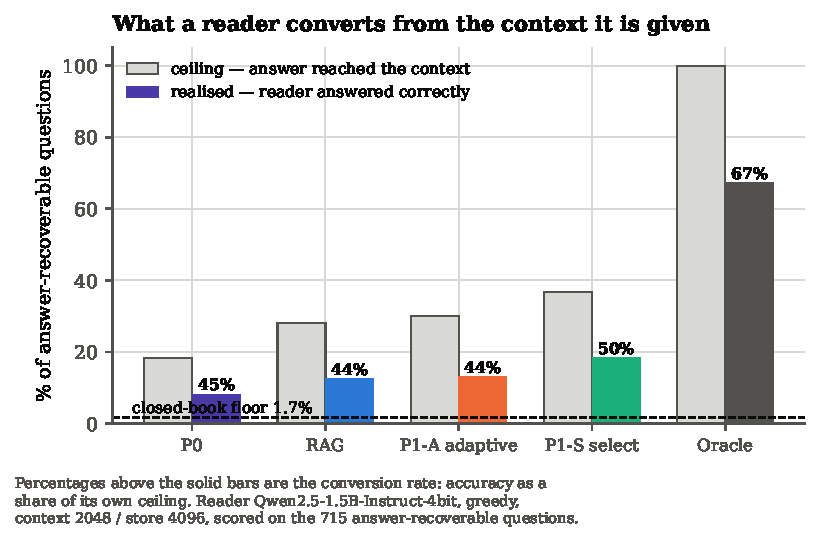
\includegraphics[width=\colfig]{figures/fig5_endtask.pdf}
\caption{Reader accuracy by memory policy, with the closed-book floor and the
oracle ceiling. The ordering matches the recall ordering, at a lower level.}
\label{fig:endtask}
\end{figure}

\subsection{Against MemGPT-style and Mem0-style memory}
\label{sec:external}

So far every baseline has been our own. To compare MemGate with designs that
people actually use, we rebuilt the memory management of MemGPT
\cite{packer2023memgpt} and Mem0 \cite{chhikara2025mem0} inside the same
harness, at the same
context budget and store budgets. The MemGPT-style arm keeps a recent queue
and a searchable archive, and folds messages evicted from the archive into a
recursive summary that is always in context and loses its oldest detail
first. The Mem0-style arm writes one compressed fact per turn with ADD,
UPDATE (the nearest stored fact above a similarity threshold is replaced,
newest wins) and NOOP for filler, and evicts the least recently touched fact.
Neither calls an LLM: summaries and facts are written by MemGate's own
extractive compressor, so these are the systems' memory structures rather
than their prompts. In the baselines' favour, each one's settings were
grid-searched on LoCoMo itself at $S=4096$ (MemGPT-style: summary share 0.25,
16-token gists; Mem0-style: 32-token facts, update threshold 0.65). No MemGate
arm was tuned on these answers.

Table~\ref{tab:external} and Fig.~\ref{fig:external} report the result. The
learned scorer beats both rebuilds at every budget, by $+7.3$ to $+24.6$
points over Mem0-style and $+11.5$ to $+22.7$ over MemGPT-style, every gap
significant under clustering. The untrained P1 heuristic beats MemGPT-style
everywhere ($+5.6$ to $+11.3$) but loses to the tuned Mem0-style at $S=4096$,
the budget its settings were chosen on, by $7.0$ points with the interval
excluding zero; it is level at 2048, ahead at 8192 by $+5.2$ (McNemar
$p=0.03$, but not significant once resampled by conversation), and well ahead
at 16384. Mem0-style stops improving at 52.6\% from $S=8192$: UPDATE replaces
a fact with its nearest neighbour, so a threshold loose enough to help at small
$S$ discards distinct facts that merely look alike, and the store never fills.
MemGPT-style stays within about two points of plain RAG, because its summary
holds gists whose answers were compressed away, the failure of
Section~\ref{sec:selection} in a different form.

\begin{table}[t]
\caption{Answer recall (\%) on LoCoMo against rebuilt MemGPT-style and
Mem0-style memory, context 2048. The baselines' settings were tuned on LoCoMo
at $S=4096$; P1-S and the held-out learned scorer P3 were not. Bold $\Delta$:
95\% interval resampled by conversation excludes zero.}
\label{tab:external}
\centering
\small
\begin{adjustbox}{max width=\columnwidth}% GENERATED by paper/make_tables.py -- do not edit by hand.
\begin{tabular}{@{}rrrrrrrr@{}}
\toprule
& & MemGPT & Mem0 & & & \multicolumn{2}{c}{$\Delta$ vs.\ Mem0-style} \\
\cmidrule(l){7-8}
$S$ & RAG & -style & -style & P1-S & P3 & P1-S & P3 \\
\midrule
2048 & 18.3 & 18.7 & 26.4 & 27.8 & \textbf{33.7} & $+1.4$ & {\boldmath$+7.3$} \\
4096 & 28.1 & 30.2 & 44.5 & 37.5 & \textbf{52.0} & {\boldmath$-7.0$} & {\boldmath$+7.6$} \\
8192 & 44.3 & 46.4 & 52.6 & 57.8 & \textbf{69.1} & $+5.2$ & {\boldmath$+16.5$} \\
16384 & 66.4 & 65.7 & 52.6 & 71.3 & \textbf{77.2} & {\boldmath$+18.7$} & {\boldmath$+24.6$} \\
\bottomrule
\end{tabular}
\end{adjustbox}
\end{table}

\begin{figure}[t]
\centering
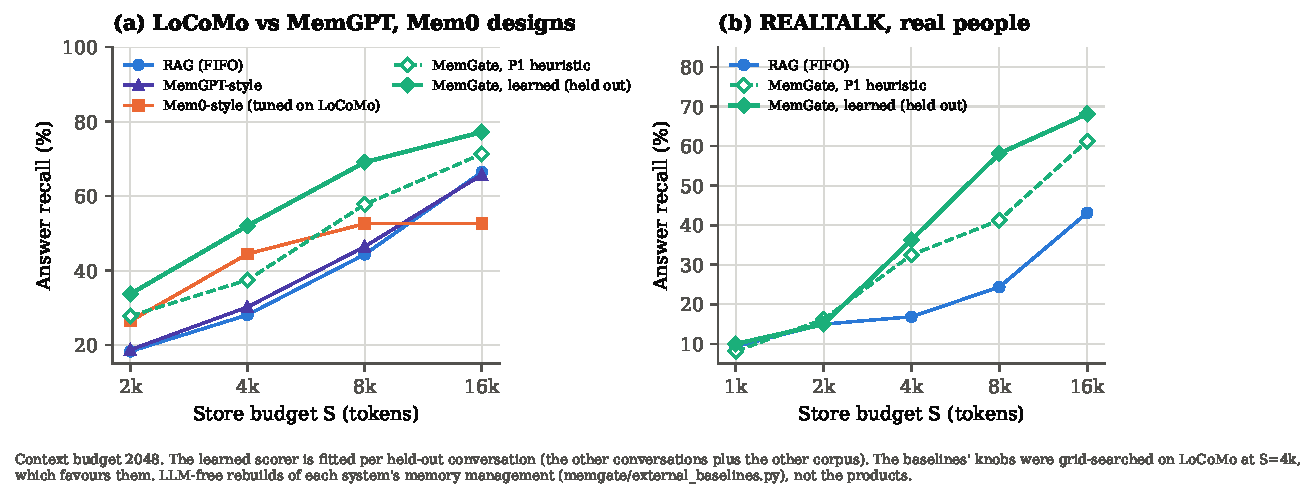
\includegraphics[width=\colfig]{figures/fig6_external.pdf}
\caption{Answer recall against the store budget for MemGate and the rebuilt
MemGPT-style and Mem0-style memories (Table~\ref{tab:external}).}
\label{fig:external}
\end{figure}

\subsection{Chats of up to ten million tokens}
\label{sec:scale}

LoCoMo conversations average about 19K tokens. BEAM
\cite{tavakoli2026beam} supplies synthetic user--assistant chats at 100K,
500K, 1M and 10M tokens with probing questions that cite turns, and MemBench
\cite{tan2025membench} short agent trajectories made of factual statements.
Two repairs were needed before BEAM 1M and 10M could be scored: some chats
restart their turn numbering partway, so each question is pinned to the
segment whose cited turns share the most words with it, and only when that
segment leads clearly. At 1M, 3 of 625 questions could not be pinned; at
10M, 128 of 200 are pinned and the rest are abstentions or cite turns that no
part of the chat holds. Each conversation is then scored by a learned
scorer fitted, under five folds by conversation, without it; BEAM 1M and 10M
are outside its training corpora altogether. The store budget is $S=26{,}000$
for BEAM, about 2.5\% of a 1M-token chat.

Table~\ref{tab:scale} reports answer recall. The learned scorer beats RAG on
all seven corpora with the interval excluding zero, by $+36.5$ points on BEAM
1M and $+46.2$ on BEAM 10M. On a million-token chat RAG keeps only the most
recent turns, so almost nothing it is asked about survives: evidence recall,
which covers 622 questions on BEAM 1M rather than 52, is 22.2\% for the
learned scorer against 0.9\% for RAG. The one corpus on which it is not the
best is MemBench, whose turns are short factual statements, which is what the
P1 rules were written to find; there P1 leads it by 1.9 answer points (n.s.).
BEAM answers are mostly paraphrases, so only a few questions per corpus are
answer-recoverable, and the BEAM 10M row rests on 13 questions.

\begin{table*}[t]
\caption{Held-out answer recall (\%) at each corpus's own store budget, 5-fold
by conversation. P3$_{12}$ is the PR~\#12 recipe (LoCoMo, REALTALK, BEAM
100K/500K), refitted without the held-out fold; P3$_{\mathrm{ship}}$ is the
shipped ensemble of Section~\ref{sec:retrain}, under the same protocol. $n$ is
the number of answer-recoverable questions. Bold: the 95\% interval, resampled
by conversation, excludes zero. $^\ddagger$PersonaChat validation dialogues,
never trained on; queries are the persona lines, a proxy described in
Section~\ref{sec:retrain}.}
\label{tab:scale}
\centering
\small
\begin{adjustbox}{max width=\textwidth}
% GENERATED by paper/make_tables.py -- do not edit by hand.
\begin{tabular}{@{}lrrrrrlrl@{}}
\toprule
Corpus & $S$ & $n$ & RAG & P1 & P3$_{12}$ & P3$_{12}-$RAG [95\% CI] & P3$_{\mathrm{ship}}$ & P3$_{\mathrm{ship}}-$P3$_{12}$ [95\% CI] \\
\midrule
LoCoMo & 4096 & 715 & 28.1 & 37.5 & 50.3 & {\boldmath$+22.2$} $[+17.5,\, +27.6]$ & 51.9 & $+1.5$ $[-0.2,\, +3.4]$ \\
REALTALK & 4096 & 160 & 16.9 & 32.5 & 36.2 & {\boldmath$+19.4$} $[+7.5,\, +26.4]$ & 36.2 & $0.0$ $[-3.3,\, +3.1]$ \\
BEAM 100K & 26K & 34 & 32.4 & 35.3 & 73.5 & {\boldmath$+41.2$} $[+14.3,\, +67.6]$ & 73.5 & $0.0$ $[0.0,\, 0.0]$ \\
BEAM 500K & 26K & 55 & 32.7 & 32.7 & 63.6 & {\boldmath$+30.9$} $[+16.7,\, +44.8]$ & 61.8 & $-1.8$ $[-10.0,\, +5.8]$ \\
BEAM 1M & 26K & 52 & 13.5 & 11.5 & 50.0 & {\boldmath$+36.5$} $[+21.8,\, +51.0]$ & 50.0 & $0.0$ $[-7.3,\, +8.0]$ \\
BEAM 10M & 26K & 13 & 7.7 & 23.1 & 53.8 & {\boldmath$+46.2$} $[+10.0,\, +76.9]$ & 38.5 & $-15.4$ $[-44.4,\, 0.0]$ \\
MemBench & 2048 & 367 & 76.8 & 97.5 & 95.6 & {\boldmath$+18.8$} $[+14.2,\, +23.7]$ & 97.5 & {\boldmath$+1.9$} $[+0.3,\, +3.8]$ \\
Everyday chat$^\ddagger$ & 1024 & 1762 & 28.8 & 30.4 & 61.4 & --- & 69.0 & {\boldmath$+7.6$} $[+5.9,\, +9.5]$ \\
\bottomrule
\end{tabular}

\end{adjustbox}
\end{table*}

\subsection{Ten times the training data}
\label{sec:retrain}

The learned scorer that the application first shipped was fitted on 58,616
turns. We retrained it on ten times that: BEAM 1M (74,630 turns) and 10M
(208,696), and MemBench's observation and participation sets, 594,000 turns
in all, with the families of Eq.~(\ref{eq:loss}) weighted equally. Each
candidate was replayed through P1-S on held-out conversations at three to
five budgets per corpus, and the whole protocol was repeated with the folds
dealt from three different orders, 26,444 replays in all. The rule for
shipping a model is that it must lose nowhere.

More data on its own did not help (Table~\ref{tab:retrain}, first column). The
10x model gains on MemBench, the corpus that was added, but loses evidence
recall on BEAM 1M by 5.1 to 5.6 points and on BEAM 500K by 3.0 to 5.2, with
the interval excluding zero in every shuffle. Our reading is that a linear
model on 399 inputs was not short of data but of capacity: the new turns are
a different kind of chat, mostly negatives (BEAM 10M adds 208,696 turns and
only a few hundred evidence labels), and they pull the weights toward short
factual statements at the cost of BEAM's long answers. Boosted trees, the
obvious source of capacity, gained on BEAM 500K but lost $8.5$ points on
LoCoMo ($[-11.1,-5.3]$) and were rejected.

Three changes put it right. The family weight of Eq.~(\ref{eq:loss}) is split
among corpora by evidence turns instead of equally, so BEAM 10M's many
unlabelled turns count for little. Everyday chat is added as a fifth family:
894 long chats assembled from PersonaChat \cite{zhang2018personachat}, 262,876
turns, weakly labelled (a turn is evidence when it states one of its
speaker's persona lines). And the result is averaged in logit space with the
earlier model, Eq.~(\ref{eq:ens}), which keeps the ranking that suited BEAM's
long answers while adding what the new chats taught, at a linear model's
cost. The shipped model is trained on 856,876 turns, 14.6 times the original.
For an everyday-chat test, 50 PersonaChat validation chats that no model saw
are replayed at $S=1024$; each stated persona line is asked as a query, and
the answer is the words of it that the person said. That is a proxy, since
query and evidence share wording, but it treats every arm alike.

At the paper's budgets the shipped model has no significant loss on any
corpus in any of the three shuffles (Table~\ref{tab:retrain}). It gains on
everyday chat ($+7.6$ to $+8.2$ answer points, 69.0\% against 61.4\%), on
MemBench, and on BEAM 100K through the application's own path ($+11.5$ to
$+12.4$ evidence points), and ties on BEAM 1M, where the 10x model lost. Across
all other budgets it has one significant loss: BEAM 1M evidence recall at
$S=8000$, $-1.7$ $[-2.8,-0.6]$, about one cited turn in sixty.

\begin{table}[t]
\caption{Retraining: change against the PR~\#12 recipe in three reshuffled
fold orders, at each corpus's budget (Table~\ref{tab:scale}), held out.
``App path'' adds the application's chunking, guard and multi-query
retrieval. Bold: the 95\% interval, resampled by conversation, excludes
zero.}
\label{tab:retrain}
\centering
\small
\begin{adjustbox}{max width=\columnwidth}% GENERATED by paper/make_tables.py -- do not edit by hand.
\begin{tabular}{@{}llll@{}}
\toprule
& 10x (594K turns) & \multicolumn{2}{c}{Shipped (857K turns)} \\
\cmidrule(lr){2-2}\cmidrule(l){3-4}
Corpus & Evidence & Answer & Evidence \\
\midrule
LoCoMo & $-0.4$, $-0.8$, $-0.2$ & $+1.5$, $-0.3$, $+0.3$ & $+0.1$, $-0.2$, $+0.2$ \\
REALTALK & $+0.1$, $-1.6$, $0.0$ & $0.0$, $0.0$, $+0.6$ & $-0.3$, $-0.8$, $+0.2$ \\
BEAM 100K & $-1.3$, $-0.8$, {\boldmath$-3.7$} & $0.0$, $+2.9$, $-2.9$ & $+1.8$, {\boldmath$+1.8$}, $+0.6$ \\
BEAM 500K & {\boldmath$-5.2$}, {\boldmath$-4.4$}, {\boldmath$-3.0$} & $-1.8$, $+1.8$, $+1.8$ & $+1.6$, $+2.0$, {\boldmath$+2.8$} \\
BEAM 1M & {\boldmath$-5.1$}, {\boldmath$-5.6$}, {\boldmath$-5.3$} & $0.0$, $-1.9$, $+1.9$ & $+0.3$, $0.0$, $-0.4$ \\
BEAM 10M & {\boldmath$-2.3$}, $-2.5$, $-0.5$ & $-15.4$, $0.0$, $-7.7$ & $-1.2$, $-1.8$, $+1.2$ \\
MemBench & {\boldmath$+5.5$}, {\boldmath$+5.8$}, {\boldmath$+6.2$} & {\boldmath$+1.9$}, {\boldmath$+1.9$}, {\boldmath$+2.2$} & {\boldmath$+5.6$}, {\boldmath$+5.9$}, {\boldmath$+6.4$} \\
Everyday chat$^\ddagger$ & --- & {\boldmath$+7.6$}, {\boldmath$+8.2$}, {\boldmath$+8.0$} & {\boldmath$+8.8$}, {\boldmath$+9.1$}, {\boldmath$+9.3$} \\
App path, BEAM 100K & {\boldmath$+6.1$}, $+4.2$, $+6.0$ & {\boldmath$+11.8$}, {\boldmath$+11.8$}, $+8.8$ & {\boldmath$+12.4$}, {\boldmath$+11.5$}, {\boldmath$+11.9$} \\
App path, LoCoMo & $-0.5$, $-0.7$, $-0.2$ & $+1.5$, $0.0$, $+0.4$ & $+0.3$, $+0.1$, $+0.5$ \\
App path, REALTALK & $+0.7$, $+0.3$, $-0.3$ & $+3.1$, $+1.9$, $+0.6$ & $+0.5$, $-0.1$, $0.0$ \\
\bottomrule
\end{tabular}
\end{adjustbox}
\end{table}

%% ======================================================================
\section{From Harness to Application}
\label{sec:system}
%% ======================================================================

The policy is not only an experiment; it also runs as a working system. A chat
application wraps a reader model in the same \texttt{observe()} and
\texttt{build\_context()} calls the experiments use (Fig.~\ref{fig:arch}).
Every message, from the user or from the model, passes through the policy, and
every question is answered from the context MemGate assembles, never from the
raw history.

The application adds one step the experiments do not have: an entry gate that
scores each message the moment it is sent. A message the scorer labels filler
(a greeting, ``ok cool'', at most two words), or a model reply scoring below
$0.1$, is forgotten straight away and never takes up space. Under P1-A and P1-S
a message with $u\ge\tau_{\text{fact}}$ is also written to Tier~3 immediately,
with its score, while staying in Tier~1 for the next few replies; when it
later leaves Tier~1, the near-duplicate rule folds it into that copy. All
other messages follow the experimental path unchanged. The gate can be turned
off, and the built-in benchmark described below runs the policies without it.

The reader can be swapped freely because it only ever receives two strings:
the assembled context and the current message. By default it runs offline on
an 8\,GB laptop with Qwen2.5-1.5B-Instruct \cite{qwen2025}. A hosted model
(Claude, or Gemini \cite{gemini2023} on its free tier) can take its place, and
if the hosted model is rate-limited and a local copy is installed, Qwen
answers that message instead. With no model at all, the application shows the
context the reader would have received. P1-S is the default policy, using the
shipped learned scorer of Section~\ref{sec:retrain} inside GuardedScorer
(Eqs.~(\ref{eq:ens})--(\ref{eq:floor}), Fig.~\ref{fig:scoring}). If the MiniLM
embedder is missing, the application falls back to the P1 heuristic instead
of scoring with the wrong features. Any text can be added. Pasted text, PDF,
Word, PowerPoint and other files are cleaned, and anything longer than 120
tokens is cut into pieces of at most 48 tokens, each scored, stored and
retrieved like a turn, because a single embedding of a long document describes
little more than its opening.

Reusing the experimental code gives two useful properties. First, persistence
is exact. A conversation is saved as its messages and restored by replaying
them through \texttt{observe()}, which is deterministic, so the tiers after a
restart match the tiers before it. Second, the application can check itself.
A built-in benchmark recomputes the RAG and P1-S arms on all of LoCoMo at
$S=4096$ on a CPU and compares them with the committed results, reproducing
28.1\% and 37.5\% exactly. A side panel shows each message's utility $u$, the
tier it went to or the reason it was forgotten, and the exact context sent to
the reader, so every decision the paper measures in aggregate can be inspected
one message at a time. The application runs at the experimental budgets by
default. It also offers a reduced scale (a Tier~1 of four messages, a
512-token context and $S=150$) at which eviction becomes visible within a few
messages. These sizes and the entry gate are the only settings that differ
from the experiments.
\subsection{Stress and scale through the application}
\label{sec:stress}

The benchmarks above replay conversations straight through the policy. To
test the system a person would actually use, whole BEAM chats were typed into the application
one message at a time, exactly as its page sends them, with each chat's
recorded assistant turns as the replies, at $S=26{,}000$. Each answerable
question was then asked as a message, and the notes each memory would hand
the reader were checked. Table~\ref{tab:appbeam} reports the result: on
million-token chats, which MemGate holds at about 2.5\%, the answer reaches
the reader for 51.9\% of questions against 19.2\% for RAG and 9.6\% for a
sliding window. The store never exceeded $S$, and a message took 0.49\,s on
average on a shared 4-core machine. This run used the PR~\#12 scorer, the one
shipped at the time; repeating it with the current one takes about ten hours
and was not done, but the held-out application-path rows of
Table~\ref{tab:retrain} are the current model's.

\begin{table}[t]
\caption{Whole BEAM chats typed into the application one message at a time,
$S=26{,}000$. $N$ chats of the given mean length in millions of tokens; $n$
answerable questions; answer recall (\%). BEAM 1M is outside the scorer's
training corpora; BEAM 500K is inside them.}
\label{tab:appbeam}
\centering
\small
\begin{adjustbox}{max width=\columnwidth}% GENERATED by paper/make_tables.py -- do not edit by hand.
\begin{tabular}{@{}lrrrrrrlr@{}}
\toprule
Chats & $N$ & M tok. & $n$ & P0 & RAG & MemGate & $\Delta$ vs.\ RAG [95\% CI] & McNemar $p$ \\
\midrule
BEAM 1M & 33 & 1.07 & 52 & 9.6 & 19.2 & \textbf{51.9} & {\boldmath$+32.7$} $[+19.2,\, +46.3]$ & $9.1\!\times\!10^{-4}$ \\
BEAM 500K & 33 & 0.52 & 55 & 12.7 & 30.9 & \textbf{65.5} & {\boldmath$+34.5$} $[+19.6,\, +49.1]$ & $3.1\!\times\!10^{-4}$ \\
\bottomrule
\end{tabular}
\end{adjustbox}
\end{table}

Much of the gap comes down to where the evidence sits. Table~\ref{tab:age} splits
LoCoMo and REALTALK questions by the position of their evidence in the
conversation. RAG forgets oldest-first, so for evidence in the first third it
keeps the answer 8--9\% of the time; the untrained P1 heuristic keeps 20--33\%,
and the learned scorer more, although on these two corpora it is in-sample
and its column is a ceiling. For evidence in the last third RAG is
competitive, since recency is then the right rule.

\begin{table}[t]
\caption{Answer recall (\%) by the position of a question's evidence in the
conversation, $S=4096$. RAG and P1 are untrained. $^\ast$The shipped PR~\#12
scorer, in-sample on both corpora.}
\label{tab:age}
\centering
\small
% GENERATED by paper/make_tables.py -- do not edit by hand.
\begin{tabular}{@{}llrrrr@{}}
\toprule
Corpus & Evidence in & $n$ & RAG & P1 & P3$^\ast$ \\
\midrule
LoCoMo & first & 262 & 9.2 & 33.2 & 51.9 \\
 & middle & 225 & 14.2 & 38.2 & 53.8 \\
 & last & 228 & 63.6 & 41.7 & 54.4 \\
\midrule
REALTALK & first & 86 & 8.1 & 19.8 & 33.7 \\
 & middle & 45 & 11.1 & 40.0 & 55.6 \\
 & last & 29 & 51.7 & 58.6 & 65.5 \\
\bottomrule
\end{tabular}

\end{table}

People rarely ask one clean question per message. When each LoCoMo question
was buried in 150--450 words of other chat, using the whole message as the
query dropped answer recall from 53.1\% to 30.3\%; joining the message's
questions into one query recovered 42.1\%, and making each question its own
query with interleaved rankings (Eq.~(\ref{eq:retrieve})) recovers 49.8\%
(REALTALK: 47.5\%, 26.2\%, 42.5\% and 43.8\%).

The same tests found six input-handling bugs, each now pinned by a test: half
of an emoji in one message made every later save of that chat fail; a 300\,KB
Word file that unzips to 300\,MB used 3.8\,GB of memory; deeply nested JSON
dropped the connection; request bodies had no size limit; a message of only
invisible characters was accepted; and a locked PDF gave an unclear error. A
load test found one more: under bursts, the server's accept queue of five
reset 314 of 2{,}000 requests from 200 simultaneous visitors. With a queue
of 256 the same test completes with no errors in 25\,s (95th percentile
2.7\,s per message), and 100 messages sent into one chat at the same moment
are all kept. A single chat of 5{,}000 messages stays at 4{,}093 of its
4{,}096 tokens, at 0.12\,s per message by the end. The one slow path left is
reopening a saved million-token chat, which replays it through memory and
takes 70\,s.

%% ======================================================================
\section{Threats to Validity}
\label{sec:threats}
%% ======================================================================

Three errors changed our results before we caught them, and in each case an
invariant caught it, not a read-through of the code. Two of the three are
forms of leakage, a well-known source of irreproducible machine-learning
results \cite{kaufman2012leakage,kapoor2023leakage}.

\emph{A policy that read its evaluation label.} LoCoMo marks every evidence
turn with a \texttt{fact\_id}, and an early consolidation rule used it to
decide what to promote. In effect the policy was reading the answer key. It
was worth 45 to 47 recall points and invalidated the first result we reported.
The fix is an invariant rather than a convention: strip every evaluation label
from the input, and the resulting store must be bit-identical. Every decision
point added since then was put under that check before it produced a number.

\emph{A component's value depends on the current bottleneck.} We first
measured the sentence embedder at $+0.2$ points and decided it hardly mattered.
That was true only where we measured it, with retrieval saturated against a
write path that threw away 93\% of the conversation. Once that bottleneck was
gone, the same swap was worth $+19.7$. An ablation run against a bottlenecked
pipeline will keep undervaluing whatever would matter once the dominant term
moves.

\emph{A failure invisible in the aggregate.} Batched judge scoring returned
\texttt{NaN} for short turns, and only for short turns. We suspected numerical
precision, but \texttt{float32} did not help. The real cause was left-padding,
which produced attention rows that were entirely masked. Without an explicit
guard, every filler turn would have scored \texttt{NaN} and turned the
eviction order upside down.

We found a fourth defect after the main runs. The heuristic scored each turn
with its speaker tag still attached, which stopped the filler rule from firing
and handed almost every turn the proper-noun bonus: 5{,}863 of 5{,}882 LoCoMo
turns were labelled facts. The recall tables and Table~\ref{tab:transfer} use
the fixed scorer; the judge, end-task, abstractive and LongMemEval runs came
before the fix. Fixing it moves the headline P1-S result from 36.8\% to
37.5\%, and shrinks the learned scorer's lead over the heuristic at $S=2048$
from $+5.2$ to $+2.7$ points, since part of that lead was the defect holding
the heuristic back.

%% ======================================================================
\section{Limitations}
\label{sec:limitations}
%% ======================================================================

\emph{Few conversations.} The conversation is the right unit for resampling,
but it leaves us with few clusters and therefore wide intervals. Effects that
do not survive are reported as not significant. REALTALK adds ten
conversations but only 160 answer-recoverable questions, too few to settle
most of its differences.

\emph{A single reader model.} Section~\ref{sec:endtask} uses one 1.5B four-bit
model \cite{qwen2025} with greedy decoding. We claim the ordering of the
policies, not their absolute accuracies. The oracle arm's 67.3\% shows that
much of the remaining error belongs to the reader. A larger reader would lift
every arm and could narrow or widen the margins, and it may also use position
in the context differently \cite{liu2024lostmiddle}.

\emph{Compression was tested in both forms.} Replacing P1-A's word selection
with a 1.5B model that rewrites each evicted turn is worth $+4.06$ answer
points (CI $[+0.84, +6.66]$), so part of the negative result was down to the
compressor rather than to compression as such. Selection still wins (pre-fix
run): 36.8\% against 34.1\%, at 2.1\,s against 3{,}892\,s and 4{,}879
generations. The claim therefore narrows: a better compressor helps, but it
does not overtake dropping.

\emph{Concatenated streams are synthetic}, as discussed in
Section~\ref{sec:scaling}.

\emph{The scorer is tuned to this corpus.} On a 94-item LongMemEval
\cite{wu2024longmemeval} subsample, whose turns average 210 tokens against
LoCoMo's 32, the heuristic's separation between evidence and non-evidence turns
flipped sign, and scored eviction lost to FIFO. The $+9.37$ of
Section~\ref{sec:selection} should be read as what a policy recovers
\emph{given a scorer suited to the corpus}, not as a property of scored
selection in general. We have since tested the learned scorer held out on
BEAM, where the heuristic also ranks evidence below chance, and on MemBench
and everyday chat (Section~\ref{sec:scale}). LongMemEval, where the
heuristic's sign first flipped, remains untested with it because we could not
fetch it in our environment. The scorer's labels are distant supervision (a
turn is positive if any question cites it), and that supervision is twice as
dense on LoCoMo (24\% of turns) as on REALTALK (12\%). On PersonaChat it is
weaker still: a word-overlap match with a persona line.

\emph{Few answerable questions at scale.} BEAM's answers are mostly
paraphrases, so only 34 to 55 questions per scale are answer-recoverable, and
13 at 10M. The intervals in Table~\ref{tab:scale} are wide as a result, which
is why we also report evidence recall, covering about ten times as many
questions. The rebuilt MemGPT-style and Mem0-style arms reproduce those
systems' memory structures without their LLM calls, so they measure the
designs rather than the products.

\emph{Single embedder and single judge.} The negative result of
Section~\ref{sec:scorer} is evidence about a 0.5B model prompted one turn at a
time, not about LLM-judged salience in general. A larger judge, or one shown
the neighbouring turns, has not been tried, and it is the most direct way to
challenge the finding.

%% ======================================================================
\section{Conclusion}
\label{sec:conclusion}
%% ======================================================================

Under the accounting this field normally uses, tiered compression loses to
storing everything and retrieving. That result is an artefact of leaving the
store unbounded. Once the store is bounded, deciding which items to forget is
worth $+9.37$ answer-recall points at identical storage, fidelity and
retrieval, while compressing an evicted item instead of dropping it costs
$7.13$. The point at which rate--distortion theory \cite{cover2006elements}
says compression should start to pay is not reached by $182\times$. Counting
the embedding index in the budget reverses the ranking below about 40\,KiB.

The obvious route to a better scorer, an LLM judge, loses to a regular
expression, and for a reason we can name: salience is not a property of a
turn read on its own. A logistic scorer over a sentence embedding, trained on
generated and human conversations together, beats the heuristic by $+14.55$
points on held-out LoCoMo conversations and by a significant margin at every
store budget from 2048 to 16384 tokens. It transfers from human dialogue to
generated dialogue, but not the other way round. Through a fixed reader,
$+6.0$ of the pre-fix $+8.7$ points survive as correct answers. The same
scorer beats MemGPT-style and Mem0-style memory, rebuilt in this harness and
tuned in their favour, at every budget we tried. On held-out chats of up to
ten million tokens it beats retrieval on every corpus, and when million-token
chats are typed into the application it keeps the answer 51.9\% of the time
against 19.2\%. Ten times the training data did not, on its own, produce a
better linear scorer. Weighting corpora by their labels, adding everyday chat
and averaging with the earlier model did, with no significant loss at the
paper's budgets.

Our practical advice is narrow: keep a scored subset at full fidelity rather
than compressing everything \cite{jiang2023llmlingua,ge2024icae}, and count
the budget in bytes with the index included. The methodological lesson is
broader. Three of the results above changed sign or size once a measurement
error was removed, and none of those errors showed up in the aggregate numbers
they distorted.

Two questions stay open. The pooled scorer's gains on human conversation
become significant only once the store holds about 40\% of a conversation,
and the scorer is untested on LongMemEval, where the hand-written cues
inverted. More human-written evidence, rather than a larger model, is what
would settle both. Second, a scorer learned online from retrieval feedback is
already statistically level with the heuristic on LoCoMo, with no labels and
no future questions ($-2.94$, n.s.). Whether it can start from the pooled
scorer and then adapt to each user is the step from a scorer fitted to
benchmarks to one fitted to the person using the application.

\section*{Acknowledgment}
The authors thank the faculty of the School of Technology Management \&
Engineering, SVKM's NMIMS, Indore Campus, for their guidance throughout this
capstone project.



\bibliographystyle{IEEEtran}
\bibliography{refs}

\end{document}
